\titlepageframe % Specific command 
%%%%%%%%%%%%%%%%%%%%%%%%%%%%%%%%%%%%%%%%%%%%%%%%%%%%%%%%%%%%%
\begin{tframe}{Introduzione}
\begin{itemize}
\item Dalla crisi del 2007 e la conseguente esplosione delle basi tra tassi di tenore differente il mercato dei derivati su tasso si è dovuto adattare a quello che è stato definito: Mondo Multi-Curva
    \begin{itemize}
    \item Esigenza di calibrare una curva di forwarding per ogni tenore
    \item Esigenza di calibrare una curva di discounting esogeno da applicare ad ogni tenore
    \end{itemize}
\item In questo contesto, poichè i collateral scambiati vengono depositati su conti che maturano interessi al tasso EONIA, la curva overnight ha assunto:
   \begin{itemize}
    \item Il compito di curva di discounting esogeno applicabile ad ogni tenore
    \item Il compito di curva di forwarding per il proprio tenore
    \end{itemize}
\item Introdurre distorsioni nella calibrazione conduce a prezzi non ragionevoli specialmente per scopi di trading, dove $1/4$ di Basis Point può fare la differenza    
\end{itemize}
\end{tframe}
%%%%%%%%%%%%%%%%%%%%%%%%%%%%%%%%%%%%%%%%%%%%%%%%%%%%%%%%%%%%%
\begin{tframe}
\begin{figure}[!h]
\centering
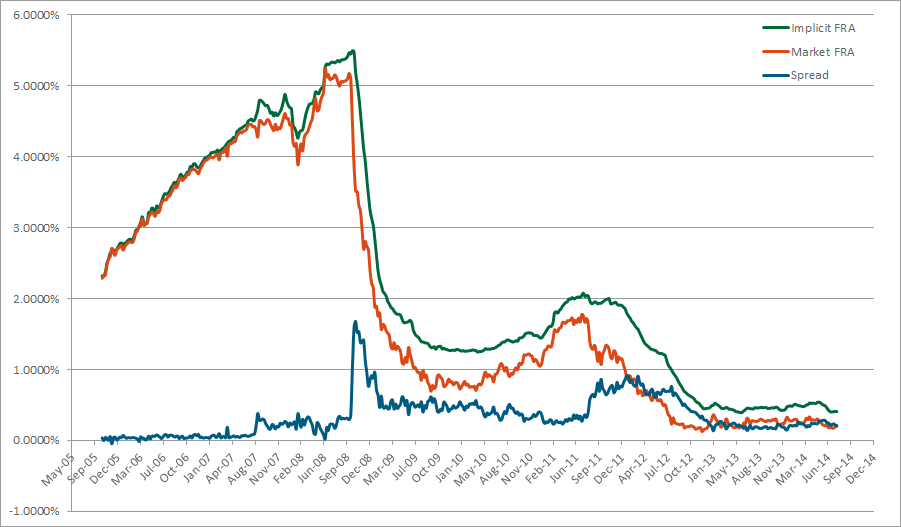
\includegraphics[width=0.8\textwidth]{basisafter}
\caption{Dopo l'estate del 2007 il  $3X6$ FRA implicito nei fixings di Euribor6M e Euribor3M non era più in linea con il $3X6$ FRA quotato sul mercato.}
\label{fig:basisafter}
\end{figure}
\end{tframe}
%%%%%%%%%%%%%%%%%%%%%%%%%%%%%%%%%%%%%%%%%%%%%%%%%%%%%%%%%%%%%
\begin{tframe}{Composizione curva Overnight}
\begin{itemize}
\item Il principio di coerenza di tenore e liquidità impone che la best practice per il bootstrap della curva overnight preveda l'inclusione di:
    \begin{itemize}
    \item Tutti forward ECB OIS disponibili sul mercato
    \item OIS con partenza spot fino a 60Y
    \end{itemize}
\item Tuttavia gli ECB OIS sono più liquidi degli OIS con partenza spot e, per questo motivo, gli algoritmi di calibrazione gli danno precedenza andando ad escludere i rispettivi spot OIS che coprono la stessa frazione di anno    
\end{itemize}
\end{tframe}
%%%%%%%%%%%%%%%%%%%%%%%%%%%%%%%%%%%%%%%%%%%%%%%%%%%%%%%%%%%%%
\begin{tframe}{Strumenti sovrapposti}
\begin{itemize}
\item Il principio di coerenza di tenore e liquidità impone che la best practice per il bootstrap della curva overnight preveda l'inclusione di:
    \begin{itemize}
    \item Tutti forward ECB OIS disponibili sul mercato
    \item OIS con partenza spot fino a 60Y
    \end{itemize}
\item Tuttavia gli ECB OIS sono più liquidi degli OIS con partenza spot e, per questo motivo, gli algoritmi di calibrazione gli danno precedenza andando ad escludere i rispettivi spot OIS che coprono la stessa frazione di anno    
\end{itemize}
\end{tframe}
%%%%%%%%%%%%%%%%%%%%%%%%%%%%%%%%%%%%%%%%%%%%%%%%%%%%%%%%%%%%%
\begin{tframe}{Installazione (II)}
In alternativa, Beamer2Thesis può essere scaricato dalla mia pagina personale come file .zip
\begin{itemize}
\item \href{http://claudiofiandrino.altervista.org/latex\_projects.html}{http://claudiofiandrino.altervista.org/latex\_projects.html}
\end{itemize}
o dalla pagina ufficiale:
\begin{itemize}
\item \href{http://cfiandra.github.com/Beamer2Thesis/}{http://cfiandra.github.com/Beamer2Thesis/}
\end{itemize}
Ovviamente deve essere installato seguendo la procedura standard di installazione manuale di un pacchetto: suggerisco, ancora di leggere la guida di Enrico Gregorio
\end{tframe}
%%%%%%%%%%%%%%%%%%%%%%%%%%%%%%%%%%%%%%%%%%%%%%%%%%%%%%%%%%%%%
\begin{tframe}{Le guide}
\begin{itemize}
\item Le slide seguenti illustrano tutte le possibili opzioni selezionabili
\item Come esempi dove le varie opzioni solo utilizzate, è possibile consultare le seguenti guide:
\begin{itemize}
\item beamer2thesis.pdf è la guida standard, in inglese, dove sono utilizzate le opzioni standard
\item beamer2thesis\_ita.pdf è la guida in italiano, con tema di colore verde e opzioni diverse da quelle standard
\end{itemize}
\end{itemize}
\end{tframe}
%%%%%%%%%%%%%%%%%%%%%%%%%%%%%%%%%%%%%%%%%%%%%%%%%%%%%%%%%%%%%
\begin{frame}[t,fragile]{Come leggere le guide}
\begin{itemize}
\item Entrembe le guide spiegano le opzioni generali; per avere una panoramica completa, potete guardare entrembe le guide, perchè in ognuna di esse è riportata la configurazione
\item Ogni volta che un'opzione è attiva o no di \emph{default}, è possibile ometterla nel premabolo
\item Ogni volta che un'opzione si attiva con \emph{true}, potete disabilitarla con \emph{false}; ad esempio:
\begin{verbatim}
secondcandidate=false 
secondcandidate=true 
\end{verbatim}
\end{itemize}
\end{frame}
%%%%%%%%%%%%%%%%%%%%%%%%%%%%%%%%%%%%%%%%%%%%%%%%%%%%%%%%%%%%%
\begin{frame}[t,fragile]{Il preambolo}
\begin{itemize}
\item \`E la prima cosa che si deve dichiarare nel preambolo
\item In generale il codice è: \verb!\usetheme[.. options ..]{TorinoTh}!
\item Ecco un esempio:
\begin{verbatim}
\documentclass{beamer}
\usetheme[language=italian,
          titlepagelogo=logopolito,
          bullet=triangle,
          pageofpages=of,
          titleline=true,
          color=green
          ]{TorinoTh}
\end{verbatim}
\end{itemize}
\end{frame}
%%%%%%%%%%%%%%%%%%%%%%%%%%%%%%%%%%%%%%%%%%%%%%%%%%%%%%%%%%%%%
\begin{tframe}{Alcune opzioni generali}
\begin{enumerate}
\item L'opzione \highlight{pageofpages} definisce una stringa fra l'attuale numero di slide e il totale
  \begin{itemize}
  \item la stringa di default usata è \emph{of}
  \end{itemize}
\item Se l'opzione \highlight{titleline} è settata a \emph{true}, una linea orizzontale viene creata sotto il titolo della slide, con il colore del tema
\begin{itemize}
  \item l'opzione per default è \emph{true}; usare \emph{false} per disabilitare
\end{itemize}
\item L'opzione \highlight{notshowauthor} definita come \emph{true} permette di non mostrare il nome dell'autore nel footer
\begin{itemize}
\item il default è \emph{false}
\end{itemize}
\item L'opzione \highlight{titlepagelogo} rappresenta il nome del logo principale: deve essere un file .jpg, .pdf, .png
\begin{itemize}
\item per includere il logo della vostra Università, seguite le procedure della prossima slide
\end{itemize}
\end{enumerate}
\end{tframe}
%%%%%%%%%%%%%%%%%%%%%%%%%%%%%%%%%%%%%%%%%%%%%%%%%%%%%%%%%%%%%
\begin{tframe}{Come inserire un nuovo logo}
Ci sono diversi modi per inserire il vostro logo (per persone molto esperte in \LaTeX\, non è certo un problema), ma suggerisco questo metodo generale:
\begin{itemize}
\item scaricate il file .zip dalla mia pagina personale ed estraetelo
\item copiate il vostro logo nella directory LaTeX (troverete già altri due loghi)
\item installate il pacchetto nel vostro albero personale seguendo la procedura standarad per installare un pacchetto (guida riportata in slide \ref{slide-guide-installation})
\end{itemize}
\label{slide-rule-installation}
\end{tframe}
%%%%%%%%%%%%%%%%%%%%%%%%%%%%%%%%%%%%%%%%%%%%%%%%%%%%%%%%%%%%%
\begin{frame}[t,fragile]{Altre opzioni: simboli per gli elenchi}
\begin{itemize}
\item L'opzione \highlight{bullet} può essere usata per selezionare il simbolo da utilizzare negli elenchi puntati
  \begin{itemize}
  \item \verb!square!: un quadrato interamente colorato
        ({\usebeamercolor[fg]{item}\tiny\raise0.2ex\hbox{$\blacksquare$}}) per elenchi con annidamento di primo e terzo livello e un quadrato bianco all'interno
        ({\usebeamercolor[fg]{item}\tiny\raise0.2ex\hbox{$\square$}}) per il secondo livello di annidamento
  \item \verb!diamond!: un rombo interamente colorato
        ({\usebeamercolor[fg]{item}\tiny\raise0.2ex\hbox{$\blacklozenge$}}) per elenchi con indentazione di primo e terzo livello e un rombo bianco all'interno
        ({\usebeamercolor[fg]{item}\tiny\raise0.2ex\hbox{$\lozenge$}}) per il secondo livello di annidamento
  \item \verb!triangle!: un triangolo interamente colorato
        ({\usebeamercolor[fg]{item}\tiny\raise0.2ex\hbox{$\blacktriangleright$}}) per elenchi con annidamento di primo e terzo livello e un triangolo bianco all'interno
        ({\usebeamercolor[fg]{item}\tiny\raise0.2ex\hbox{$\vartriangleright$}}) per il secondo livello di annidamento
  \item \verb!circle! (default): un cerchio interamente colorato
        ({\usebeamercolor[fg]{item}\tiny\raise0.2ex\hbox{$\bullet$}}) per elenchi con annidamento di primo e terzo livello e un cerchio bianco all'interno
        ({\usebeamercolor[fg]{item}\tiny\raise0.2ex\hbox{$\circ$}}) per il secondo livello di annidamento
  \end{itemize}
\end{itemize}
\end{frame}
%%%%%%%%%%%%%%%%%%%%%%%%%%%%%%%%%%%%%%%%%%%%%%%%%%%%%%%%%%%%%
\begin{frame}[t,fragile]{Lingue}
\begin{itemize}
\item Tutte le lingue sono disponibili, ma le due principali sono:
\begin{itemize}
\item inglese
\item italiano
\end{itemize}
\item La scelta di una delle due lingue principali implica che, nella pagina iniziale, date e label (Supervisor, Candidate, Relatore, Candidato) siano riportate esattamente in modo automatico
\item Per selezionare la lingua italiana, ad esempio, usate nel preambolo:
\verb!language=italian!
il nome deve essere quello utilizzato dal pacchetto babel or dal comando \verb!\setmainfont! con \XeLaTeX
\item Se la lingua selezionata non è una delle due principali, occorre ridefinire manualmente le label del frontespizio (si riporta un esempio nella diapositiva successiva)
\end{itemize}
\end{frame}
%%%%%%%%%%%%%%%%%%%%%%%%%%%%%%%%%%%%%%%%%%%%%%%%%%%%%%%%%%%%%
\begin{frame}[t,fragile]{Lingue (II)}
\begin{itemize}
\item Un esempio con la lingua spagnola:
\begin{verbatim}
\usetheme[language=spanish,...]{TorinoTh}
\setrellabel{Relator Tesis}
\setcandidatelabel{Candidato}
\setassistentsupervisorlabel{Co Tesis}
\setsubject{Tesis}
\end{verbatim}
\item I comandi illustrati sono obbligatori quando \highlight{non si utilizza} una delle due lingue principali
\item Se avete scelto una lingua e volete cambiarla, può succedere che, la prima compilazione dia questo errore: \begin{flushleft}
\highlight{! Package babel Error: You haven't loaded the option -lingua- yet}
\end{flushleft}
non spaventatevi e compilate nuovamente: funzionerà!
\end{itemize}
\end{frame}
%%%%%%%%%%%%%%%%%%%%%%%%%%%%%%%%%%%%%%%%%%%%%%%%%%%%%%%%%%%%%
\begin{frame}[t,fragile]{Codifica}
Per non forzare l'utente ad utilizzare esclusivamente la codifica utf8x, questa versione risolve il problema introducendo l'opzione \highlight{coding}; le possibili scelte sono:
\begin{itemize}
\item \verb!coding=utf8x! (default)
\item \verb!coding=utf8!
\item \verb!coding=latin1!
\end{itemize}
Un avviso: il programma non controlla eventuali errori di inserimento ed è compito del lettore assicurarsi di scegliere la giusta codifica che il suo sistema richiede.
\end{frame}
%%%%%%%%%%%%%%%%%%%%%%%%%%%%%%%%%%%%%%%%%%%%%%%%%%%%%%%%%%%%%
\begin{frame}[t,fragile]{Secondo logo}
\begin{itemize}
\item Se è necessario inserire un secondo logo (ad esempio per una tesi di laurea con doppio titolo), un'opzione permette di visualizzarlo nella pagina iniziale
\item Quando l'opzione \highlight{secondlogo} è \emph{true}, dovete utilizzare il comando \verb!\titlepagesecondlogo{name-logo}! per inserire il logo: se non è presente si verifica un errore
\item Come il logo principale, anche il secondo logo deve essere un'immagine in .jpg, .pdf, .png, e, potete inserirlo, utilizzando le stesse regole spiegate nella slide \ref{slide-rule-installation}
\end{itemize}
\end{frame}
%%%%%%%%%%%%%%%%%%%%%%%%%%%%%%%%%%%%%%%%%%%%%%%%%%%%%%%%%%%%%
\begin{frame}[fragile]{Terzo logo}
\begin{itemize}
\item Eventualmente, se è necessario un terzo logo, avete la possibilità di inserirlo settando l'opzione \highlight{thirdlogo} a \emph{true}
\begin{itemize}
\item il default è \emph{false}
\end{itemize}
\item L'immagine deve essere caricata seguendo le procedure descritte per il primo e secondo logo; poi utilizzate il comando \verb!\titlepagethirdlogo{name-logo}! per inserire il logo nel frontespizio
\item Naturalmente, potete usare questa opzione se, e solo se, anche il \highlight{secondlogo} è \emph{true}
\item Quando inserite tre loghi usate, come riferimento per le dimensioni, la figura \alert{logopolito}: in questo modo risulteranno perfettamente allineati
\end{itemize}
\end{frame}
%%%%%%%%%%%%%%%%%%%%%%%%%%%%%%%%%%%%%%%%%%%%%%%%%%%%%%%%%%%%%
\begin{frame}[t,fragile]{Secondo candidato}
\begin{itemize}
\item \`{E} possibile che in una tesi ci siano due candidati: Beamer2Thesis gestisce con facilità questo caso
\begin{itemize}
\item il \emph{primo} candidato è anche l'autore
\item il secondo candidato viene inserito con il comando \verb!\secondcandidate{nome-cognome}! quando l'opzione \highlight{secondcandidate} è \emph{true}
\end{itemize}
\item Naturalmente, in presenza di due candidati, la label \emph{Candidate} diventa \emph{Candidates} e la label \emph{Candidato} diventa \emph{Candidati}
\item Con due candidati, il footer cambia e l'autore non viene mostrato (la ragione è semplice: due autori più il titolo rendono il footer troppo grande)
\end{itemize}
\end{frame}
%%%%%%%%%%%%%%%%%%%%%%%%%%%%%%%%%%%%%%%%%%%%%%%%%%%%%%%%%%%%%
\begin{frame}[t,fragile]{Relatore e Correlatore}
\begin{itemize}
\item Per inserire il relatore è sufficiente usare il comando \verb!\rel{nome-cognome}!
\item Inoltre, è possibile inserire il correlatore:
\begin{itemize}
\item settando l'opzione \highlight{assistantsupervisor} a \emph{true} (il default è \emph{false})
\item usare il comando \verb!\assistantsupervisor{nome-cognome}!
\end{itemize}
\item Le label sono inserite in base alla lingua selezioanta
\end{itemize}
\end{frame}
%%%%%%%%%%%%%%%%%%%%%%%%%%%%%%%%%%%%%%%%%%%%%%%%%%%%%%%%%%%%%
\begin{frame}[t,fragile]{Secondo Relatore e Correlatore}\label{secondrel}
Esiste la possibilità di inserire un secondo relatore e correlatore:
\begin{itemize}
\item grazie alle opzioni:
\begin{itemize}
\item \highlight{secondsupervisor} settato a true (default is false)
\item \highlight{secondassistantsupervisor} settato a true (default is false)
\end{itemize}
\item i nomi possono essere inseriti con:
\begin{itemize}
\item il comando \verb!\secondsupervisor! per il relatore
\item il comando\verb!\secondassistantsupervisor! per il correlatore; in questo caso, si può utilizzare questo comando soltanto se l'opzione \highlight{assistantsupervisor} è true
\end{itemize}
\item come sempre, le label si aggiornano correttamente a seconda della lingua scelta e al plurale
\end{itemize}
\end{frame}
%%%%%%%%%%%%%%%%%%%%%%%%%%%%%%%%%%%%%%%%%%%%%%%%%%%%%%%%%%%%%
\begin{frame}[t,fragile]{Vantaggi e Svantaggi}
A volte è utile evidenziare vantaggi e svantaggi di un determinato argomento: anzichè elencarli con gli ambienti normali, esiste la possibilità di impiegare due nuovi ambienti (\emph{adv} and \emph{disadv}). Il metodo di utilizzo è il seguente:
\begin{columns}
\begin{column}{0.3\paperwidth}
\begin{verbatim}
\begin{adv}
\item 
\end{adv}
\end{verbatim}
\end{column}
\begin{column}{0.3\paperwidth}
\begin{verbatim}
\begin{disadv}
\item 
\end{disadv}
\end{verbatim}
\end{column}
\end{columns}
\bigskip
Nella slide seguente è riportato un esempio.
\end{frame}

\begin{tframe}{Perchè usare Beamer2Thesis}
Vantaggi:
\begin{adv}
\item Semplice da installare
\item Facile la personalizzazione
\item Possibilità di utilizzare diverse funzionalità
\end{adv}
Svantaggi:
\begin{disadv}
\item Difficile gestione di titoli enormemente lunghi
\item Se trovate altri svantaggi.. contattatemi
\end{disadv}
\end{tframe}

\begin{frame}[t,fragile]{Infine i colori}
\begin{itemize}
\item Esistono tre possibili sfumature cromatiche:
\begin{itemize}
\item blu
\item verde
\item rosso
\end{itemize}
\item La sfumatura desiderata viene scelta con l'opzione \highlight{color} dalla lista precendente e, di conseguenza, sono definite intestazioni di inizio e piè di pagina, il frontespizio, i simboli degli elenchi e i colori di evidenziazione del testo
\item Ad esempio: \verb!color=green!
\end{itemize}
\end{frame}

\begin{tframe}{\XeLaTeX}
Grazie ad un suggerimento e al prezioso aiuto di Nicola Tuveri, Beamer2Thesis supporta \XeTeX\, and \XeLaTeX\, automaticamente.
Pertanto potete scegliere il vostro font preferito per personalizzare ulteriormente la presentazione. Ecco alcuni esempi:\\
\highlight{Rimuovere il commento seguenti righe di codice se si utilizza \XeLaTeX!}
%%% commented by Karol Kozioł
%\fontspec[Ligatures={Common, Historical}]{Linux Libertine O Italic}
%\fontsize{12pt}{18pt}\selectfont Questo è strano! 
%\fontspec{TeX Gyre Pagella}
%\selectfont{Anche questo è strano}\\
%\fontspec[ SizeFeatures={
%{Size={-10}, Font=TeX Gyre Bonum Italic, Color=AA0000},
%{Size={10-14}, Color=00AA00},
%{Size={14-}, Color=0000FA}} ]{TeX Gyre Chorus}
%\selectfont{Come personalizzare i font?}\par
%\begin{itemize}
%\item {\LARGE Parola}
%\item Parola
%\item {\tiny Parola}
%\end{itemize}
\end{tframe}

\begin{frame}[t,fragile]{\XeLaTeX\,: il codice}
Per realizzare gli esempi riportati nella slide precedente, il codice da utilizzare è:
\scriptsize{
\begin{verbatim}
\fontspec[Ligatures={Common, Historical}]{Linux Libertine O Italic}
\fontsize{12pt}{18pt}\selectfont Questo è strano! 
\fontspec{TeX Gyre Pagella}
\selectfont{Anche questo è strano}\\
\fontspec[ SizeFeatures={
{Size={-10}, Font=TeX Gyre Bonum Italic, Color=AA0000},
{Size={10-14}, Color=00AA00},
{Size={14-}, Color=0000FA}} ]{TeX Gyre Chorus}
\selectfont{Come personalizzare i font?}\par
\begin{itemize}
\item {\LARGE Parola}
\item Parola
\item {\tiny Parola}
\end{verbatim}
}
\end{frame}

\begin{tframe}{Block}
Beamer permette di utilizzare gli ambienti \emph{block}: sono molto comodi in alcune applicazioni. Per esempio:
\begin{block}<1->{Perchè usare Beamer2Thesis? Vantaggi}
\begin{adv}
\item Semplice da installare
\item Facile la personalizzazione
\item Possibilità di utilizzare diverse funzionalità
\end{adv}
\end{block}
\begin{block}<2->{Perchè usare Beamer2Thesis? Svantaggi}
\begin{disadv}
\item Difficile gestione di titoli enormemente lunghi
\item Se trovate altri svantaggi.. contattatemi
\end{disadv}
\end{block}
\end{tframe}

\begin{frame}[t,fragile]{Block: codice}
La slide precedente è stata realizzata con il seguente codice:
\small{\begin{verbatim}
\begin{block}<1->{Perchè usare Beamer2Thesis? Vantaggi}
\begin{adv}
\item Semplice da installare
\item Facile la personalizzazione
\item Possibilità di utilizzare diverse funzionalità
\end{adv}
\end{block}
\begin{block}<2->{Perchè usare Beamer2Thesis? Svantaggi}
\begin{disadv}
\item Difficile gestione di titoli enormemente lunghi
\item Se trovate altri svantaggi.. contattatemi
\end{disadv}
\end{block}
\end{verbatim}}
\end{frame}

\begin{frame}[t,fragile]{Block: codice (II)}
Più in generale, Beamer offre la possibilità di utilizzare tre ambienti \emph{block}:
\begin{itemize}
\item \highlight{block}
\item \highlight{alertblock}
\item \highlight{exampleblock}
\end{itemize}
Per avere più dettagli, e non solo su questo argomento, suggerisco di leggere la \href{http://mirrors.ctan.org/macros/latex/contrib/beamer/doc/beameruserguide.pdf}{beameruserguide}.
\end{frame}